%%%%%%%%%%%%%%%%%%%%%%%%%%%%%%%%%%%%%%%%%%%%%%%%%%%%%%%%%%%%%%%%%%%%%%%%%%%%%%%
%                     Отчёт по лабораторной работе №6
%
% Дисциплина: Теория вероятностей и Математическая статистика
%                     
% Название:   Простая линейная регрессия
%
% Выполнил:   Михаил Маляренко
%
% Дата:       12 Янв. 2021
%
%%%%%%%%%%%%%%%%%%%%%%%%%%%%%%%%%%%%%%%%%%%%%%%%%%%%%%%%%%%%%%%%%%%%%%%%%%%%%%%

% HEADER BEGIN 
\documentclass[12pt]{article}
\usepackage[utf8]{inputenc}
\usepackage[russian]{babel}
\usepackage{pscyr}
\usepackage[T2A]{fontenc}
\usepackage{geometry}
\usepackage{graphicx}
\usepackage{multirow}
\usepackage{hhline}
\usepackage{amsmath}
\usepackage{amssymb}
\usepackage{hyperref}
\usepackage{xcolor}

\geometry {	
	a4paper, 
	left   = 20mm, 
	right  = 20mm, 
	top    = 20mm, 
	bottom = 20mm
}

\definecolor{urlcolor}{HTML}{2484BC} 
\definecolor{linkcolor}{HTML}{000000}

\graphicspath{{resource/}}
% HEADER END

% DIFINES BEGIN
\newcommand{\lskip}{\hfill\break}
% DEFINES END

\begin{document}

\begin{titlepage}
	\begin{center}
		\hfill \break
		{\textbf{Санкт-Петербургский политехнический университет Петра Великого}}\\
		\hfill \break
		\textbf{Институт прикладной математики и механики}\\
		 \hfill \break
		\textbf{Кафедра <<Телематика (при ЦНИИ РТК)>>}\\
		\vfill
		\large{\bfseries Отчет по лабораторной работе}\\
		\hfill \break
		\hfill \break
		\hfill \break
		\hfill \break
        \normalsize{\bfseriesПростая линейная регрессия}\\
        \hfill \break
		По дисциплине <<Теория вероятностей и Математическая статистика>>\\
		\hfill \break
		\hfill \break
	\end{center}
 
	\normalsize
	{ 
		\begin{tabular}{lp{2cm}cr}
			Выполнил &&&\\
			Студент гр. 3630201/80101&&\underline{\hspace{1.5cm}}& М. Д. Маляренко\\\\
			Руководитель&&&\\ 
			к.ф.-м.н., доцент && \underline{\hspace{1.5cm}}& А. Н. Баженов \\\\
			&&&<<\underline{\phantom{333}}>>\underline{\phantom{сентября000}}
			2020г.
		\end{tabular}
	}
\vfill

\begin{center} Санкт-Петербург \\2020 \end{center}
\end{titlepage}

\newpage

\setcounter{page}{2}

\begin{flushleft}

\setlength{\parindent}{1cm}

% TABLE OF CONTENTS
\tableofcontents

\newpage

% LIST OF FIGURES
\listoffigures

\newpage

\section{Постановка задачи}
Найти оценки коэффициентов линейной регрессии $y_i = a + bx_i + e_i$, используя 20 точек на отрезке [-1.8; 2] с равномерным шагом равным 0.2.
Ошибка $e_i$ распределена по стандартному нормальному закону $N(0, 1)$.
В качестве эталонной зависимости взять $y_i = 2 + 2x_i + e_i$.
При построении оценок коэффициентов использовать два критерия: 

\begin{enumerate}
	\item Критерий наименьших квадратов
	\item Критерий наименьших модулей
\end{enumerate}
Проделать то же самое для выборки, у которой в значения $y_1$ и $y_{20}$ вносятся возмущения 10 и -10.

\newpage

\section{Теория}

\subsection{Простая линейная регрессия}

    \subsubsection{Модель простой линейной регрессии}
    Регрессионную модель описания данных называют простой линейной регрессией, если
    \begin{equation}
        y_i = \beta_0 + \beta_1x_i + \varepsilon_i, \quad i=1, \dots, n,
    \end{equation}
    где $x_1, \dots, x_n$ — заданные числа (значения фактора); $y_1, \dots, y_n$ — наблюдаемые значения отклика; $\varepsilon_1, \dots, \varepsilon_n$ — независимые, нормально распределённые $N(0,\sigma)$ с нулевым математическим ожиданием и одинаковой (неизвестной) дисперсией случайные величины (ненаблюдаемые); $\beta_0, \beta_1$ — неизвестные параметры, подлежащие оцениванию.

    \subsubsection{Метод наименьших квадратов}
    Метод наименьших квадратов (МНК) \cite{theory}:
    \begin{equation}
        Q(\beta_0, \beta_1) = \sum_{i = 1}^{n}\varepsilon_{i}^{2} = \sum_{i = 1}^{n}(y_i - \beta_0 - \beta_1x_i)^2 \rightarrow \min_{\beta_0, \beta_1}.
    \end{equation}

    \subsubsection{Расчётные формулы для МНК-оценок}
    МНК-оценки параметров $\beta_0$ и $\beta_1$ \cite{theory}:
    \begin{equation}
        \hat{\beta}_1 = \frac{\overline{xy} - \overline{x} \cdot \overline{y}}{\overline{x^2} - (\overline{x})^2}
        \label{mnk1}
    \end{equation}
    \begin{equation}
        \hat{\beta}_0 = \overline{y} - \overline{x}\hat{\beta}_1
        \label{mnk0}
    \end{equation}

\subsection{Робастные оценки коэффициентов линейной регрессии}
Метод наименьших модулей \cite{theory}:
\begin{equation}
    \sum_{i = 1}^{n}|y_i - \beta_0 - \beta_1x_i| \rightarrow \min_{\beta_0, \beta_1}.
\end{equation}
\begin{equation}
    \hat{\beta}_{1R} = r_Q\frac{q^{*}_{y}}{q^{*}_{x}},
    \label{mnm1}
\end{equation}
\begin{equation}
    \hat{\beta}_{0R} = med \; y - \hat{\beta}_{1R} med \; x,
    \label{mnm0}
\end{equation}
\begin{equation}
    r_Q = \frac{1}{n}\sum_{i=1}^{n}sgn(x_i - med \; x)sgn(y_i - med \; y),
\end{equation}
\begin{equation}
    q^{*}_{y} = \frac{y_j - y_l}{k_q(n)}, \qquad q^{*}_{x} = \frac{x_j - x_l}{k_q(n)}
\end{equation}
\[
    l = 
		\left\{
		\begin{aligned}
			 \left[n/4\right] + 1& \;\; \text{при} \;\; n/4 \;\; \text{дробном,}\\
			 n/4                  & \;\; \text{при} \;\; n/4 \;\; \text{целом.}\\
		\end{aligned}
		\right.
\]
\[
    j = n - l + 1.
\]
\[
    sgn \; z = 
		\left\{
		\begin{aligned}
			 1 & \; \text{при} \; z > 0,\\
             0 & \; \text{при} \; z = 0,\\
             -1 & \; \text{при} \; z < 0.\\
		\end{aligned}
		\right.
\]
Уравнение регрессии здесь имеет вид
\begin{equation}
    y = \hat{\beta}_{0R} + \hat{\beta}_{1R}x.
\end{equation}

\newpage

\section{Реализация}

Расчёты и построение графиков производились в среде аналитических вычислений Maxima с графической оболочкой wxMaxima.
Для нахождения параметров $\beta_0, \beta_1, \hat{\beta_0}, \hat{\beta_1}$ по формулам (\ref{mnk1}), (\ref{mnk0}), (\ref{mnm1}), (\ref{mnm0}) были написаны функции \texttt{LSM} для МНК и \texttt{LMM} для МНМ. Исходный код скрипта для Maxima представлен в репозитории на GitHub. Графики были построены с помощью интегрированной утилиты \texttt{gnuplot}. 

\newpage

\section{Результаты}

	\subsection{Выборка без возмущений}

	В результате оценки параметров линейной регрессии для выборки без возмущений были получены следующие значения коэффициентов:

	\begin{itemize}
		\item МНК: $\hat{\beta}_0 \approx 2.05 \quad \hat{\beta}_1 \approx 2.06$
		\item МНН: $\hat{\beta}_{0R} \approx 1.65, \quad \hat{\beta}_{1R} \approx 1.54$
	\end{itemize}

	На Рис. \ref{reg1} представлен график модели, точки выборки, а также графики линейной регрессии с коэффициентами вычисленными по МНК и МНН.

	\begin{figure}[h]
		\center{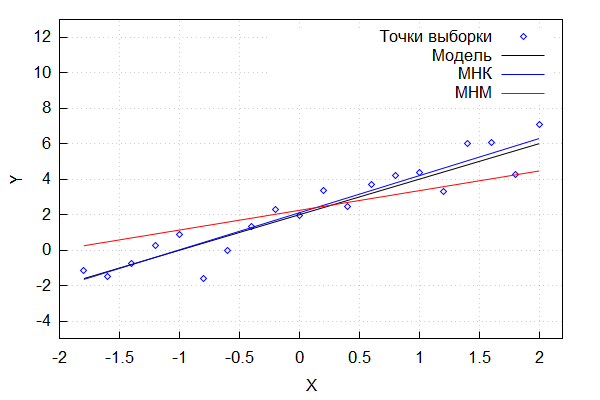
\includegraphics[width=0.8\linewidth]{regression_1.png}}
		\caption{Выборка без возмущений}
		\label{reg1}
	\end{figure}

	\newpage

	\subsection{Выборка с возмущениями}

	В результате оценки параметров линейной регрессии для выборки с возмущениями в крайних элементах были получены следующие значения коэффициентов:

	\begin{itemize}
		\item МНК: $\hat{\beta}_0 \approx 1.97, \quad \hat{\beta}_1 \approx 0.73$
		\item МНН: $\hat{\beta}_{0R} \approx 2.04, \quad \hat{\beta}_{1R} \approx 1.68$
	\end{itemize}

	На Рис. \ref{reg2} представлен график модели, точки выборки, а также графики линейной регрессии с коэффициентами вычисленными по МНК и МНН.

	\begin{figure}[h]
		\center{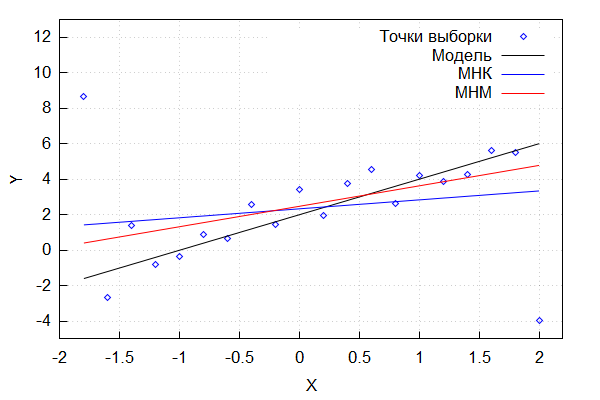
\includegraphics[width=0.8\linewidth]{regression_2.png}}
		\caption{Выборка с возмущениями}
		\label{reg2}
	\end{figure}

\newpage

\section*{Заключение}
\addcontentsline{toc}{section}{Заключение}

В результате лабораторной работы были вычислены коэффициенты линейной регрессии по методам наименьших квадратов и наименьших модулей. Как видно из оценки коэффициентов регрессии а также по графикам, метод наименьших квадратов более точен на выборке без возмущений, но уступает по точности методу наименьших модулей на выборке с редкими, но значительными выбросами.

Можно сделать вывод, что для выборок с небольшими выбросами для нахождения коэффициентов линейной регрессии предпочтительнее использовать МНК, а для выборок с большими выбросами следует использовать МНМ как менее точный, но более устойчивый.

\newpage

\addcontentsline{toc}{section}{Список литературы}
	\begin{thebibliography}{1}

		\bibitem{theory}
		Теоретическое приложение к лабораторным работам №5-8 по дисциплине «Математическая статистика». -- СПб.: СПбПУ, 2020. -- 22 c 

	\end{thebibliography}

\newpage

\section*{Приложение А. Репозиторий с исходным кодом}
\addcontentsline{toc}{section}{Приложение А. Репозиторий с исходным кодом}

Исходный код скрипта для среды аналитических вычислений Maxima находится в репозитории GitHub -- URL \url{https://github.com/malyarenko-md/TeorVer}

\end{flushleft}

\end{document}